
I have implemented a simulated surface vessel and a non-buoyant subsurface vessel, both of which are controllable either manually or by automated controller. The two vessels are bound together by a wire tether. The vessels and the wire are all affected by weather effects such as ocean currents, as well as physical effects like added mass and inertia. 

The simulation works as would be intuitively expected. An example of the simulation graphical interface can be seen in \cref{fig:sim-display}. The figure shows a surface vessel and the ROV under water in green, and the teal tether connecting them. The simulated water is shown as a grey volume, but it's not easy to distinguish it in \cref{fig:sim-display} because it takes up the entire screen. 

\begin{figure}
	\centering
	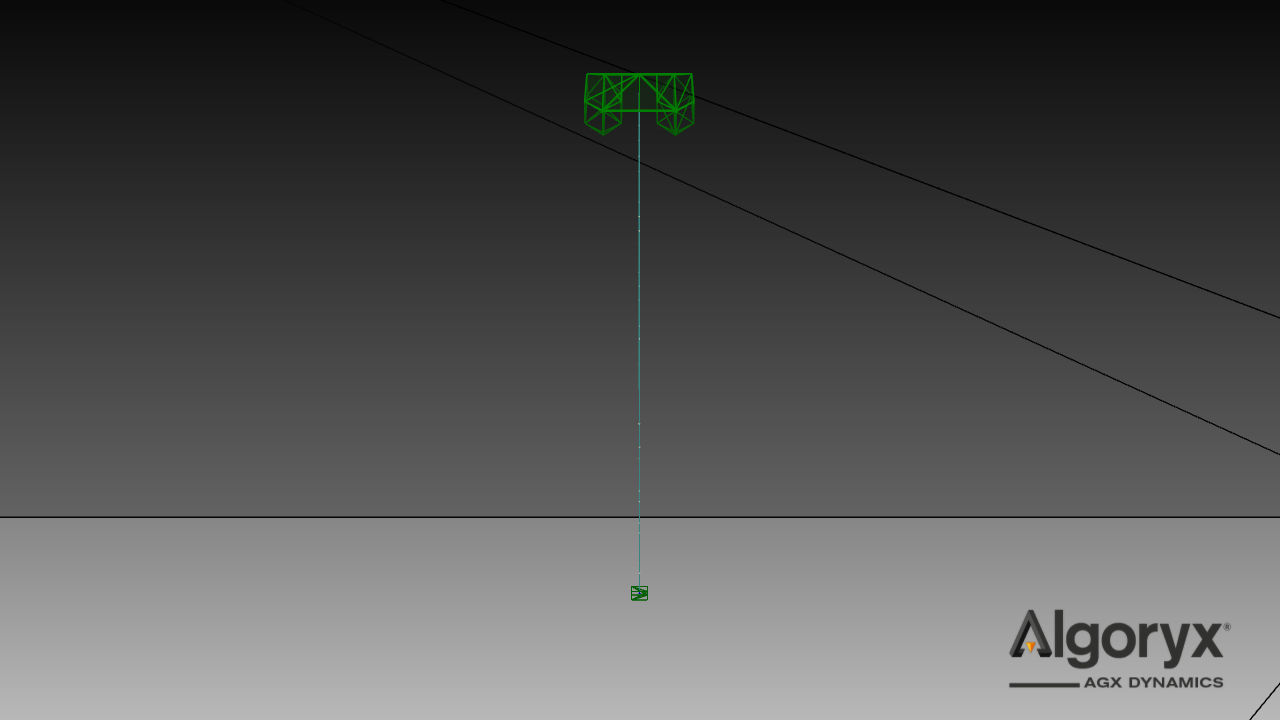
\includegraphics[width=0.7\textwidth]{sim-display}
	\caption{The graphical user interface of AGX with the simulation running}
	\label{fig:sim-display}
\end{figure}

\section{Model Validation}
\label{sec:validation}
There are two ways I will attempt to validate the simulator results here. One is intuitively and the other is using analytical methods and a couple of simple cases. The intuitive demonstration is difficult to convey in text-form in a report, but I have placed some animations of the results on GitHub\cite{noauthor_fordypogmastersimulator_nodate} along with the project. The intuitive demonstrations consist of starting the simulation, pulling objects around and seeing if they "act right". Human minds are excellent pattern recognition machines, and I will use this to my advantage here, as if something is "off", it would be noticable. 

\subsection{Intuitive validation}
I have done two tests here, one where I pull the surface vessel and look at how the ROV follows, and the other where I pull the ROV and see how the surface vessel follows. The shape of the tether is also relevant here. Looking at the results, shown in the \texttt{Results} directory of the simulator on the Github repo, there is nothing that pops out as obviously wrong. Of note is that the surface vessel flips in the ROV pulled test. This is because I pulled the ROV down and given the situation the surface vessel was in it was more stable flipped upside down. This is not a realistic scenario for the real-life project because the amount of force exerted pulling the surface vessel down will never be that large. Looking at the tension in the tether at the ROV it reaches upwards of 20kN at points, which corresponds to roughly 20 tonnes lifted.

In addition to the two tests above I've also tried swinging the ROV as a pendulum underneath the surface vessel. This test also confirms the intuitive assumption that when the surface vessel is far more massive than the ROV, it will be less affected when pulled like this, although it will still be affected. 

\subsection{Analytical validation}
For the analytical part of the validation I will use some simple cases. The first case is a towing, where the surface vessel moves forward towing the ROV behind it. This will be roughly analogous to how the ROV and tether will respond in currents. I can analytically find an expected tension in the tether and then compare this with the simulation results. I will ignore the effects of the tether for simplicity. This will be a source of error on the final result as the tether will have an effect in the simulation.

The tension on the tether in the towing case will be dependent on the resistance of the water around the tether and ROV as well as the effect of gravity. This gives the equation 
\[F = F_g + F_D\]
Where \(F\) is the total force pulling on the wire, \(F_g\) is the force due to gravity and \(F_D\) is the drag force. 

For the force of gravity I will assume that gravity is in-line with the tether. This is not the case as the ROV will lag behind a bit, causing effectively a cosine error. From having looked at the simulations this seems to be a fairly small error and so I will ignore it, but this will add to the cause of error in results. The force of gravity on the ROV simply becomes 
\[F_g = m \times g \approx 131kg \times 9.8\frac{m}{s^2} \approx 1300N\] 

The ROV will be the largest influence here due to its large size compared to the wire. The resistance for an object in a fluid (drag) is given by the equation 
\[F_D = \frac 1 2 \rho v^2 C_D A\]
Where \(F_D\) is the drag force, \(\rho\) is the density of the fluid, \(v\) is velocity, \(C_D\) is the coefficient of drag and \(A\) is the cross-sectional area. The seawater used in the simulation has defined \[\rho = 1025\frac{kg}{m^3}\] For the cross-sectional area I will assume that the ROV doesn't turn as it flows. It likely will, which will change both \(A\) and \(C_D\), but for these calculations I will ignore this. I will assume that \[A = 0.45m\times 0.254m = 0.114m^3\]

The drag coefficient of a cube is according to tables 1.05, while the drag coefficient of a square prism perpendicular to flow is 2.05. The ROV is simulated as a simple box which is roughly half of a cube, divided horizontally. I believe the actual coefficient of drag on the simulated ROV will be somewhere between these and I will use both values to calculate an upper and lower bounds. 

That only leaves the velocity as a variable. I will do simulations in increments of 1m/s from 0 to 5m/s, which is roughly 10 knots. 

\begin{table}
\begin{tabular}{c c c}
Velocity (m/s) & Calculated tension (N) & Simulated tension (N) \\
\hline
0 & & 5021 \\
1 & & \\
2 & & \\
3 & & \\
4 & & \\
5 & &
\end{tabular}
\caption{Tensions in the tether between the surface vessel and the hanging ROV}
\label{tab:tension}
\end{table}




\section{Control system results}
